\documentclass[10pt,letterpaper,twocolumn,twoside]{rho-class/rho}
%TODO: Make this 9pt after progress reports are done.
\usepackage[english]{babel}
\usepackage{longtable}
\ExecuteBibliographyOptions{sorting=none}
\DeclareBibliographyCategory{cited}
\AtEveryCitekey{\addtocategory{cited}{\thefield{entrykey}}}
% ================= MAIN DOCUMENT =================

% Restore normal page style (rho class defaults)
%\pagestyle{plain} % or whatever rho expects; remove if rho sets this itself
%TODO: Uncomment the above when done with progress reports.
% Switch back to two-column layout as specified by rho
%\twocolumn
%TODO: Uncomment the above when done with progress reports.
%----------------------------------------------------------
% Title
%----------------------------------------------------------

% \doctype{Capstone Report}
\title{\textbf{Performing a taxonomy-informed semantic reconciliation of the W3C Data Privacy Vocabulary to surface implementation considerations, decision points, and issues.}}

%----------------------------------------------------------
% Authors, Affiliations and dates
%----------------------------------------------------------

\author[{\textasteriskcentered},a,1]{\textbf{Brice Dobson}, \textit{Georgia Institute of Technology}, Atlanta, GA, USA}

%----------------------------------------------------------

%\affil[a]{The Georgia Institute of Technology}

%----------------------------------------------------------

%\dates{Version 1.0 - \today}

%----------------------------------------------------------
% Corresponding author-, Document- information
%----------------------------------------------------------

%\corres{\textsuperscript{\textasteriskcentered}Corresponding author: \href{mailto:author.one@institute.org}{author.one@institute.org} (A. One).}
%\corres{\textsuperscript{\textdagger}These authors contributed equally to this work.}

%----------------------------------------------------------

%\docinfo{This document class was prepared on Overleaf and compiled with pdf\LaTeX{}. No errors were found during the compilation process. Rho-class supports external editors, though additional setup may be required.} 

%----------------------------------------------------------

\journalname{PUBP 6727}
\journal{Version 1.0}
\theday{This file was compiled on \today}
%\vol{DRAFT}
%\no{DRAFT}

%----------------------------------------------------------
% Abstract and Keywords
%----------------------------------------------------------

\begin{abstract}
Large organizations with multi-jurisdictional privacy obligations manage significant volumes of privacy-relevant information across many process subdomains. Frequently, these organizations look to external frameworks, taxonomies, or ontologies to inform the design of these process subdomains. These frameworks often feature high internal validity but have low semantic compatibility with what is around them. Further, there is no overarching data model focused on harmonizing the work occurring within one subdomain with related concepts in adjacent subdomains, despite their data entities being inherently related in principle and practice. The result is that large organizations are left to draw compliance conclusions from data that is insufficiently precise, normalized, or complete for the purpose, ultimately representing not only a compliance risk, but a maturity ceiling in the face of a bona fide desire to comply.
\newline
This paper asks what a truly unified data model for privacy would look like for a large organization if the interoperability across its constituent process domains (subdomains) were forced. Using a canonical ontology as a foundation, the W3C Data Privacy Vocabulary, a reference data model was constructed that forced this interoperability and expands on the DPV by an order of magnitude. The work of constructing this reference model highlighted entities and relationships that are invariant multi-jurisdictionally and represent fundamental flaws of understanding and compatibility when modified, a methodology to support maturity keying and explicit consideration of the data model rework points associated with improving process maturity over time, over 40 opportunities to make latent decisions explicit to better align risk appetite and tolerance within the implementing organization, and an approach for extension of regulation-specific entities and relationships. 
    
\end{abstract}

%----------------------------------------------------------

\keywords{Data Privacy, Privacy Ontology, Privacy Taxonomy, Privacy Operations, Privacy Data Model, W3C DPV, CMMI}

%----------------------------------------------------------

\defbibfilter{taxonomyonly}{keyword=taxonomy}
\defbibfilter{taxonomystandards}{keyword=taxonomy and keyword=standards}
\defbibfilter{taxonomyregulatory}{keyword=taxonomy and keyword=regulatory}
\defbibfilter{taxonomycommercialtools}{keyword=taxonomy and keyword=commercial}
\defbibfilter{taxonomyacademicwork}{keyword=taxonomy and keyword=academic}
\defbibfilter{referencesonly}{not keyword=taxonomy}

\begin{document}
\setcounter{page}{1}

    \maketitle
    \thispagestyle{firststyle}

%----------------------------------------------------------
\phantomsection
\hypertarget{toc}{}
\setcounter{tocdepth}{2}
\tableofcontents
\label{sec:0}

\section{Introduction}\label{sec:intro}
Organizations, especially larger ones with multi-jurisdictional privacy compliance imperatives, implicitly manage many seemingly disparate categories of privacy-relevant information. These include inventories and data flows, processes and activities, purposes and lawful bases, notices, consent records, invocations of individual rights information, and formal assessments of compliance, harms, and risks. If we consider privacy an overarching process domain within an organization, each of these manifest as subdomains. Each subdomain has between several and many externally frameworks and taxonomies available for reference and implementation. These are inherently grounded in regulatory expectations, representing reasonable approaches for an organization to structure their processes and data within that subdomain. While they may be internally valid within their respective subdomains, organizations quickly experience interoperability problems in a messy middle where semantic incompatibilities arise, causing a myriad of potential issues for the implementing organization, especially as it grows and matures its process design and execution. 

The difficulties that arise from managing privacy-relevant data coherently is not attributable to any single actor but rather at the convergence of four. 
\begin{enumerate}
    \item Governments who legislate and enforce regulation.
    \item Standards bodies that seek to further interpret, operationalize, and standardize requirements
    \item Large organizations who seek to advance their missions and comply with law and regulation in the process.
    \item Commercial tool and service providers who seek to capitalize on the opportunities created by these conditions.
\end{enumerate}

\begin{figure}
    \centering
    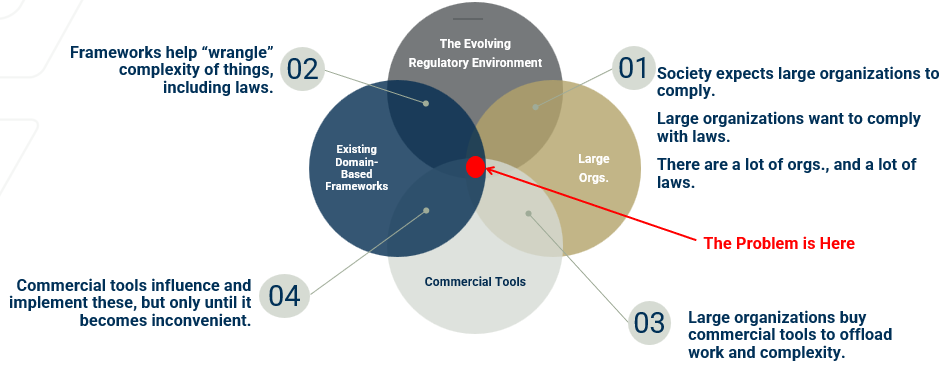
\includegraphics[width=1.0\linewidth]{Convergence.png}
    \caption{Enter Caption}
    \label{fig:placeholder}
\end{figure}

Regulations typically stop short of codifying the full relationships of the concepts they govern. Independent standards are scoped and publish at inconsistent levels of analysis and often with limited consideration for interoperability. Large organizations operationalize under internal resource and knowledge constraints and commercial tools implement solutions that implicitly and sometimes unknowingly resolve decision points that proxy for risk tolerance, often favoring their own convenience. 

Disconnected taxonomies and data models produce inconsistent terminology and data, this results in duplication without clear authority and unrecognized or unclear relationships. Organizations then rely on the resulting data to draw conclusions in contexts where that data is not sufficiently precise, normalized, or complete for the purpose. This creates a vulnerable condition for operational and legal compliance failure modes such as exceeding purpose specification in ways that erode lawful bases, inadequate recognition and fulfillment of individual rights, and missed opportunity through poor application of legal requirements. I approach this in a data-first manner with the assertion that there is a level of data normalization where these linked-but-incompatible process subdomains become compatible, and that in a well-run privacy program, drift from that normalized form should be a deliberate function of maturity targets and formally accepted risk, not an accident of tooling or organizational structure. 
\newline
This paper represents a question \emph{What would a truly unified data model for privacy look like for a large organization, if interoperability across its constituent process domains were forced?}
\newline
This problem cannot be solved through a fixed schema, because the structure inherently varies with the organization's target and actual process maturity, its portfolio of regulatory mandates, and its risk tolerance. The solution must instead be a parameterized structure with robust consideration for extension, typing, and the implicit decisions arising from accounting of entities and relationships that are inherently expressions of risk tolerance. In short, a reference data model.

This work manifests in four artifacts. 
\begin{enumerate}
    \item A reference data model spanning 12 privacy capability subdomains, comprising 34 core entities, 65 core relationships, and 12 reified-association classes, connected by 87 cross-subdomain joins and layered for regulation, maturity, and risk.
    \item An enumeration of 40 latent decision points that organizations are currently resolving implicitly, often without recognizing that they are accepting risk in doing so. 
    \item The identification of 13 gaps in the DPV, of which 10 are substantively improved upon in this work.
    \item The fourth is a machine-readable serialization of the model together with an interactive web-based explorer, evaluated through 100 SPARQL-validated test cases over 12 refinement iterations.
\end{enumerate}. 

The remainder of this paper proceeds as: Section~\ref{sec:background} establishes the regulatory, organizational, and standards conditions that motivates the work. Section~\ref{sec:method} describes the phased methodology by which the model was derived and evaluated. Section~\ref{sec:model} presents the reference model itself, including its analytic underpinnings. 
Section~\ref{sec:lqfw} states limitations, qualifications, and future work, and Section~\ref{sec:conclusion} concludes.

\section{Background}\label{sec:background}

This section contextualizes problem space and provides foundational knowledge for this work, examining each of the four actors before characterizing the ontological starting point.

\subsection{The evolving regulatory environment}\label{sec:regenv}

At least 144 countries now have laws addressing privacy and data protection obligations of organizations~\cite{IAPP144}. These take similar but not perfectly compatible approaches, split between comprehensive and sectoral models, and regulators are often unconcerned if the law they enforce creates a compliance issue under another regulatory regime. Simultaneously, individuals are becoming more aware of their rights as data subjects, with industry reporting a 128\% increase in individual rights request rates per million identities in just a two-year period~\cite{Cisco2026}. Enforcement is widening in parallel, with the early actions grounded in data security issues and breach giving way to lawful basis and individual rights issues, which now represent one-third and one-quarter of known GDPR enforcement actions respectively~\cite{CMS2025Numbers}.

\subsection{Independent standards bodies}\label{sec:standards}

Independent standards bodies occupy the space between the regulators who define required outcomes and the organizations expected to produce them. Institutions such as ISO/IEC, IEEE, and the W3C convert broad legal duties into defined recommended practice through consensus processes, member review, and published revision cycles. This deliberateness of authorship is what establishes their credibility which translates to authority over time. While the authority of these bodies is persuasive rather than coercive, regulators lean on standards to give operational meaning to ambiguous legal requirements, with the GDPR's ``state of the art'' security obligation being a canonical example~\cite{gdpr}, because referencing an evolving standard spares the law from codifying technical detail it could not keep current. 

While adoption of any independent standard is typically voluntary and does not convey or constitute legal compliance, large organizations use standards as a shared vernacular that transfers across most jurisdictions and business units. Further, these function as an attractive mechanism to signal reasonable effort, since no single regulator or vendor could or would credibly provide this assurance. Their adoption, especially under explicitly certifiable frameworks such as ISO/IEC 27701~\cite{iso27701} serve as

Commercial tool providers build to standards as de facto requirements catalogs and market their alignment, which propagates the standard's choices into implementations at scale and can be offered as a product feature.

\subsection{Large organizations}\label{sec:largeorgs}

My position is that the largest organizations absorb this, although they are still undeniably accountable to adhere to all applicable laws as a function of their costs of doing business. The top 100 multinational enterprises average more than 500 affiliate companies across more than 50 countries~\cite{unctad-top100}, and it is reasonable to assume each affiliate generates personal data compliance obligations in some context. Even organizations that could support legal teams in every country (and they often cannot) would not thereby assure compliance, given the technological detail involved and privacy's highly contextual nature. Further, over half of privacy programs are run out of legal departments~\cite{IAPP2024Gov}, with the implication that the value of data structure and a technology backbone for compliance may not be fully appreciated within the function that owns it. In parallel, privacy-related spending is accelerating. The share of large organizations spending more than \$5 million USD annually on privacy grew from 14\% to 38\%, and 93\% of organizations with at least one dedicated privacy professional report plans to increase privacy and data governance investment over the next two years~\cite{IAPP2024Gov}.

\subsection{Commercial privacy tools}\label{sec:comtools}

Commercial tool providers aim to fill the void created by the regulatory landscape and organizational desires to comply. These tool publishers play a needed role and offer the prospect of real value for their customer's money, especially for lower-maturity organizations faced with the challenge of creating something from nothing in order to get better at privacy, as they aim to reduce their exposure and risk.

However, commercial tool providers experience several practical constraints to perfect data structures within their tools, resulting in a functional parsimony in their features relevant to this problem.
\begin{itemize}
    \item Their products are expected to be usable across a wide range of customer maturity levels. That is, a mid-market enterprise in a lightly regulated industry and a high-regulated Fortune 100 large enterprise must rely on the same core data structures.
    \item There is limited appreciation for technical correctness for the sake of technical correctness, especially when it comes at the cost of usability.
    \item Technical correctness may increase complexity, thereby increasing potential for: rework, reduced stability, and administration costs.
    \item They must make a profit.
    
\end{itemize}

The net result of these is that the vendor is actually managing the data model for organizations who implement these commercial tools, and that data model makes many decisions that may be latent or unrecognized at thet ime of purchase, where a subset of these carry risk implications the implementing organization never explicitly accepted. Further, the degree that extensibility of the data model is supported may create an invisible maturity ceiling, where the organization desires to extend its data model but cannot due to feature limitations. While my assertion is not that commercial tool publishers intentionally create these ceilings in their products, it is fair to acknowledge that commercial tool providers' interests are not perfectly aligned with those of their customers.

\subsection{Ontologies, taxonomies, and schemas, oh my!}\label{sec:ontologies}

There are hundreds of ontologies, taxonomies, and other references written on how to perform selected tasks in data privacy, where these are understood to suggest either explicit or implicit data relationships. I suggest these are authored by sources that can be broadly characterized in four types; independent standards organizations, governmental or regulatory institutions, commercial organizations, and academic institutions. While not the fault of any author, by virtue of not being subject to harmonization in most cases, each body of work inherently has a different level of analysis because they are scoped through charter and developed through consensus, not an individual organization's needs. Further, interoperability with related external concepts (i.e. those outside of the explicit scope of the implied data structure) is not a widely seen  feature or requirement of these. The result is that these issues may be invisible within the domain because the data relationships implied through the standard are fully valid from that vantage (internal validity). However, the resulting incompatibility becomes visible when the organization attempts to operate several of these at once within adjacent process subdomains in data privacy. Lastly, a notable exception would be standards authored by independent standards organizations, which do regularly possess this feature of cross-subdomain compatibility, although this is almost always exclusively offered to other standards of their shared authorship.

No one has made a comprehensive reference data model, although the most foundational single framework in this space is the World-Wide Web Consortium (W3C) Data Privacy Vocabulary (DPV)~\cite{dpv}. This is a credible ontology that seeks to explain the interactions between organizations and regulations for data privacy. It publishes concept schemes for personal data, purposes, processing operations, legal bases, entities, risk, technical and organizational measures, and rights, together with a light layer of object properties connecting them. An ontology, fundamentally, shows the interactions between things. The DPV does this well, and this work takes the position that its foundational data relationships are correct for its level of analysis. It is an excellent basic starting point, and any solution in this space is aided by resembling it.

However, ontologies generally, and the DPV specifically, lack attribute-level detail, which makes them less suitable for off-the-shelf implementation within an organization. The distinction matters because a vocabulary answers ``what concepts exist and what may relate to what,'' while an implementing organization must answer ``which records are first-class, what identifies them, which relationships are mandatory, and what happens to them over time.'' These are different questions, and conflating them is the root of common failure modes examined in Section~\ref{sec:model}.

\subsection{Where the DPV stops}\label{sec:dpvstops}

Before this work performed any extraction, the DPV was examined as if it were schema-complete, to surface the points where ambiguity in structure would otherwise pass into an implementation. The examination yielded eight categorical gaps, G1 through G8, summarized in Table~\ref{tab:gaps}.

Four of the eight concern static structure. The DPV expresses that a processing activity \emph{may have} a purpose, but never how many it must have, whether one is required, or whether multiplicity is bounded, and these are cardinality commitments any record system must make (G1). No commitment exists as to what identifies an instance of a concept, leaving keys, uniqueness constraints, and the distinction between a category and an occurrence to implementers (G2). Concept schemes do not constrain attribute datatypes, ranges, or formats, so conformance cannot be validated without first being defined (G7). And the vocabulary takes no position on which records must exist for a program to be conformant, leaving the floor undefined (G8).

The other four relate to change over time. Most DPV concepts carry no states or transitions, yet nearly every operational record moves through draft, active, suspended, and retired states with rules about which transitions are permitted (G3). These assertions carry no from/until semantics by default, making it impossible to answer ``which legal basis applied on this date,'' a question regulators ask routinely (G4). Further, there is no mechanism for representing the change history of an entity or assertion, which defeats any automated monitoring control or audit engagement that seeks to reconstruct past activity or states (G5). Lastly, metadata cannot attach to a relationship without promoting the relationship to a node, an acknowledged problem (G6).

\begin{table}[ht]
\centering
\caption{The eight categorical gaps (G1--G8) between the DPV and an implementable schema.}
\label{tab:gaps}
\footnotesize
\begin{tabular}{@{}l p{0.2\linewidth} p{0.56\linewidth}@{}}
\hline
Gap & Concern & Commitment left to the implementer \\
\hline
G1 & Cardinality & How many of each related concept must or may exist \\
G2 & Identity & What identifies an instance, including keys, uniqueness, and category versus occurrence \\
G3 & Lifecycle & Which states a record moves through and which transitions are valid \\
G4 & Temporal validity & When an assertion holds (from/until semantics) \\
G5 & Versioning & How change history is represented and reconstructed \\
G6 & Edge provenance & How metadata attaches to a relationship (promotion to a node) \\
G7 & Enforceable typing & Datatypes, ranges, and formats permitting mechanical validation \\
G8 & Mandatory records & Which records must exist for a conformant program \\
\hline
\end{tabular}
\end{table}

These are not asserted to be flaws in the DPV. They are issues largely implicit to the application of ontologies in a discrete manner. However, disregarding any one of these eight gaps during an implementation is guaranteed to result in an underdeveloped data model, because each reflects a choice that will be made somewhere, whether explicitly by the implementer or implicitly by whatever tool(s) adopt the data model.

\subsection{Maturity, regulation, and risk}\label{sec:axes}

In short, the gap between the DPV and an operating data model cannot be closed by a single fixed schema, because the correct structure is a function of three independent variables. The first is \emph{target maturity}. For this work, we ground in CMMI, using the continuous representation, where each privacy capability subdomain carries its own level (L1--L5) rather than the organization holding a single rating. Informally, L1 describes ad hoc, individually-held practice. L2 describes managed practice with records that exist as maintained data. L3 describes defined practice with records connected to a common organizational structure. L4 describes quantitatively managed practice whose records carry history, validity, and provenance sufficient for measurement. L5 describes optimizing practice where those records feed automated monitoring and improvement. The data model manifestations of L4 (versioning, immutable histories, temporal validity) would be unnecessary counterproductive overhead at L1, which is why maturity must parameterize the model rather than the model presuming a single maturity level.

The second variable is the \emph{regulatory portfolio}. A single processing activity may be simultaneously subject to GDPR, CCPA/CPRA, LGPD, and sectoral obligations, and no single regime deserves to be privileged as canonical. The third is \emph{risk tolerance}, because a meaningful set of design choices have no single correct answer and ultimately resolved against the organization's risk tolerance and appeite, as a function of how detailed the organization desires to be on a particular configuration decision. Together, these three variables define the design problem the reference model must solve, and the reason its answer must be parameterized rather than prescriptive.

\section{Methodology}\label{sec:method}

The reference data model was produced through a phased approach where each phase delivered an input to the subsequent phase. This allowed successive phases to increase abstraction (supporting data structure normalization) over the project and mitigated issues originating from premature optimization. This pipeline's output is the evaluated model presented in Section~\ref{sec:model}. At a high level, the phases were 1) preparation of the DPV skeleton and definition of subdomain boundaries, 2) identification and scoring of input taxonomies, 3) extraction of implied data entities, attributes, and relationships within these taxonomies, 4) normalization within each subdomain, 5) cross-subdomain joining, 6) technical evaluation, and 7) final reconciliations and application decisions. Table~\ref{tab:phases} summarizes the key figures produced at each phase.

\begin{table}[ht]
\centering
\caption{Methodology key figures by phase.}
\label{tab:phases}
\footnotesize
\begin{tabular}{@{}p{0.40\linewidth} p{0.46\linewidth}@{}}
\hline
Phase & Result \\
\hline
1 -- Prepare DPV skeleton & 12 subdomains defined \\
2 -- Identify input taxonomies & 40 accepted, +9 supplemental \\
3 -- Extract entities, attributes, relationships & 578 unique implied relationships (approx.\ 480 raw entries) \\
4 -- Normalize per subdomain & 160 candidate gaps and decision points, 36\% average compression \\
5 -- Cross-subdomain joins & 87 joins mapped \\
6 -- Technical evaluation & 100 test cases over 12 runs, approx.\ 12\% footprint change \\
7 -- Final reconciliation & 2 gaps raised to the W3C \\
\hline
\end{tabular}
\end{table}
TODO: Come back to this table and clean up.
\subsection{Preparing the DPV skeleton and defining the subdomains}\label{sec:skeleton}

The DPV, as an ontology, does not consider object attributes, typing, or keys, and it must be prepared to receive these during operationalization. This requires the creation of boundaries that form domains of related concepts, where the number of two-way cross-boundary relationships should be minimized. The model leans heavily on the DPV's module structure to define its subdomains, representing the process areas within a privacy program at a large organization who implements the data model. However, decomposing the DPV's module structure would have left common operational processes and artifacts without a home, including but not limited to Notice, Incident, and Regulatory Filing, as these are not first-class DPV modules. This resulted in a twelve-subdomain structure, enumerated in Table~\ref{tab:subdomains}. A thirteenth candidate, Technology \& AI Governance, was considered and set aside on the grounds that its regulatory environment remains insufficiently stable to source authoritatively, and this is revisited in Section~\ref{sec:futurework}. This also happens to align to this doamin's current status within the most current DPV, where it has been contemplated and drafted, but not at the same depth as others entities and relationships.
TODO: Add a table here with the DPV domains to remove the reference.

\subsection{Characterizing the DPV and identifying structural requirements}\label{sec:gapledger}

As described in Section~\ref{sec:dpvstops}, the DPV was examined as if schema-complete before any extraction of entities or relationships was performed, producing the eight categorical gaps G1--G8. I once again emphasize that these gaps were \textit{mostly} not the result of deficiencies in the DPV's design, but those associated with and arising from implementing ontologies as data models generally. This approach, that is enumerating these structural issues prior to any analysis of individual entities or relationships, was intentional. Specifically, its purpose was to create a series of checks that could be applied at each phase to ensure that decision points were not being inherited or remaining latent but rather being explicitly decisioned as a result of this work. This had the additional benefit of seeding the initial decision register. 

TODO: Make a table for this, possibly in the appendix.

\subsection{Identifying authoritative sources per subdomain and scoring them}\label{sec:sources}

Input taxonomies, that is the sources which provide the raw material of data entities, relationships, and attributes for the data model, were identified through research targeted at subdomain/author-type pairs. It is important to note that these sources may not have be explicitly labeled as ontologies, taxonomies, or reference data models. Rather, they represent commonly accepted ways to structure processes to perform tasks within their subdomain and had the common thread of being detailed enough in that endeavor that they explicitly and implicitly defined the most common data entities, relationships, and attributes required for the tasks they purported to standardize. The author typing approach asserted that credible authors could be classed into four groups 1) independent standards organizations, 2) governmental or regulatory institutions, 3) commercial organizations, and 4) academic institutions. For each pair, searches were conducted using keywords (e.g., ``taxonomy,'' ``ontology,'' ``classification system'') through internet search engines and bibliographic databases. Identified input taxonomies were coded by the subdomain(s) where they were suspected to imply relevant data entities, attributes, and relationships, then scored using a qualitative three-tier rating system for domain relevance, level of authority, and potential yield to the data structures of the reference model. Some input taxonomies were eliminated at this stage for having low potential yield, whether through low quality or a lack of implied data structures, or for being a summarization of another, more authoritative source of near-identical information. Selecting up to approximately the top three per subdomain produced approximately 45 accepted input taxonomies, with approximately 10 supplemental sources, where some sources served multiple subdomains. The full listing and subdomain mapping appear in Appendices B and C. TODO: Add links to appropriate appendicies.

\subsection{Extracting the structure each source implies}\label{sec:extraction}

Each source was analyzed for the entities, attributes, relationships, states, and cardinality constraints it explicitly stated. Many sources, especially those within the governmental or regulatory institutions author category, were observed to hold short of declaring requirements for data structures directly but proxy these through use-case-specific taxonomies, examples, templates, or written content. Where these implicit items could be deduced, they were captured based on the entities they implicated. Notably in the governmental or regulatory institutions author type, there was a class of input taxonomies that were preliminary identified as among the highest quality and most authoritative sources that were ultimately set aside with limited benefit. These were best characterized as "example reports", where the authors, almost exclusively regulatory enforcement authorities, were representing a presentation view of synthesized data relationships that they would expect to see in their context, rather than the underlying data relationships. An common example of this is the GDPR Article 30 report, TODO: Finish example.  

Fundamentally, the productive insight of the extraction phase is that the data model of a regulation or standard often sits in implicit form within its operational guidance. Fields contained within mandatory disclosures, retention schedules, and template forms constitute primary evidence of required data and structure. In total, 578 unique relationships were implied across the source set.

\subsection{Normalizing within each subdomain}\label{sec:normalization}

Per-source extractions were synthesized within subdomains into a single subdomain model prior to any cross-subdomain joins being mapped. While there was an early expectation that duplicates be removed, there were a number of small semantic differences that required reconciliation. These were essentially concepts that had common and often near identical definitions in plain language, but used different terminology to summarize them across different sources TODO: Add example. These were initially reconciled at this stage, but would be a theme throughout the work and are now understood to be table stakes of this type of forced-fitting approach . Basic checks were also performed at this stage to ensure a consistent level of normalization had been applied to each subdomain's data structures. Where disagreements between two or more entries were identified, these were resolved within the subdomain at this stage, and decisions related to duplication, disagreement, and cardinality were noted for each entry.

This step matters because sources disagree more than their individual authority would suggest, with over 100 disagreements documented across the corpus, concentrated on cardinality, lifecycle, primary-entity designation, and taxonomy composition. This highlights earlier assertions that each input taxonomy was authored to satisfy only its own scope, and reconciliation across sources is typically not within that scope. For implementers, this deferral can have real implications tangential to organizational forces and pressure, which creates an opportunity for latent, inconsistent, or otherwise poor decision making to infiltrate the data strucdture.

\subsection{Cross-subdomain joining}\label{sec:joining}

Upon completion of entity-relationship mapping within subdomains, cross-subdomain joins were mapped using the DPV module relationships as a loose foundation, and work items place-held from individual subdomain views were then reconciled. This produced approximately 80 cross-subdomain joins and resulted in the first draft of the full model. It also surfaced a set of ``messy middle'' artifacts that matter operationally but either lack a clear home or near-evenly span multiple process subdomains. A common theme was that most of these are instantiated, so each instance appears as a subdomain-local entity until forced to confront cross-subdomain joins. Examples include \texttt{AccountabilityArtefact} (spanning 23 typed document subtypes), \texttt{Notice}, and \texttt{ImpactAssessment}. These become first-class unifying classes in the model and are discussed in Section~\ref{sec:crosscut}.

\subsection{Evaluation}\label{sec:eval}

The evaluation approach focused primarily on the internal validity of the model, as external validity faced some constraints at this stage with time, level of effort, and information access required. I generally consider that internal validity here means the technical accuracy and completeness of the data model, where external validity is the data model's fit for use and application in implementing organizations.

For the internal validity pillar, the data model was declared as a hybrid OWL/RDFS ontology in turtle (.ttl) format, essentially making it machine-readable and compatible with common ontological tool sets. One hundred test cases were then built, informed by the NIST Privacy Workforce Taxonomy~\cite{nist-pwt-2024} and the IAPP Privacy Operational Lifecycle~\cite{iapp-ppm-2022}, representing common tasks performed in large-organization privacy programs. Each test case was written in plain language as one or more satisfaction claims, and each claim was then translated into a SPARQL (TODO: Add citation for SPARQL) SELECT query. SPARQL was selected over relational alternatives because ontologies and their tooling natively support the more complex join patterns, such as tuples, that are pervasive in this problem space. The compiled test cases were run through a custom purpose-specific Python schema validator informed by a selection of criteria from (Todo: add reference to the existing ontology handbook source) built using rdflib. The validator applied test cases that checked for likely missing entities, format gaps, missing relationships, missing attributes, typing gaps, mismatched domains, and mismatched output ranges.

One representative test case asserts the satisfaction claim \emph{``for a given processing activity, return the lawful basis in force on a specified date, together with the party that held the controller role at that time.''} (TODO: Could we add the full code snippet of the satisfaction claim here) Its SPARQL translation exercises two reified associations (\texttt{LegalBasisAssignment} and \texttt{PartyRoleInActivity}), their temporal validity attributes, and two cross-subdomain joins in a single query. A claim of this shape is unanswerable against the unimplemented DPV and within many commercial tools. This not because the concepts are missing, but rather the missing feature manifestation of the earlier highlighted gaps, specifically G4  and G6 (todo: Add parenthetical names for G4 and G6). The test suite is, in effect, a mechanized probe of whether the model technically correct, complete, and closes the original foundational gaps that were asserted as necessary for practitioner use. 

Running the suite began an iterative process (run the validator, resolve apparent issues, run it again) that converged at approximately 10 iterations. At this point, the remaining outstanding issues that remained were those that were reserved reserved for the implementer (Section~\ref{sec:risk}) and represented their stylistic choices of approach and risk tolerance, rather than the construction of the data model. The model's footprint changed approximately 15\% between the pre- and post-evaluation states, with results mostly "building out" cross-domain relationships and necessary reified entities in the "middle" of the data model. I assert this degree of change establishes the initial evaluation was substantive rather than confirmatory.

For the qualitative pillar focused on the data model's fit for use and application of the, I considered several factors that would have been constraining to the quality of this work, ultimately opting to take a limited approach in this space at this stage. These factors included but were not limited to:

\begin{enumerate}
    \item There may be less than 5,000 organizations who would have appropriate justification to implement such an approach. While other organizations beyond this may certainly benefit from this on a piecemeal basis, we must broadly consider that organizations do not seek to "do better" at legal compliance for the sake of artfulness.
    \item Exploratory conversations with stakeholders from likely candidate organizations highlighted the need to first, but near-simultaneously, qualify the problem for the organization. While it is likely that any candidate organization meeting certain size and geographic minimum criteira could benefit from this work, recognizing a bona fide need for the value (through elimination of rework and pain) of implementing such a data model is a real prerequisite for quality of evaluation and implementation.
    \item The individual who is able to qualify the intersection of the problem space and the organization is not necessarily the individual who can evaluate the data model's fit for use and application on behalf of the organization.
    \item Such an evaluation could take several to several dozen hours per evaluator/organization. Lesser attempts at this would create potential to undermine rigor in evaluation and introduce anecdotes that could errode internal validity.
    \item 
\end{enumerate}

More broadly, we consider that the approach used to construct the data model inherently selected for valid sources. That is, almost all input taxonomies were themselves subject to standalone reviews by their respective authoring entity (e.g. standards bodies, regulators, etc.) which often included formal development processes, expert evaluation, public preview and feedback, and other rigorous tactics. The model therefore inherits a meaningful degree of external validity from its sources, in the sense that its raw material was already heavily vetted, even though the composed whole has not yet received equivalent scrutiny. 

Lastly, I did approach the W3C DPV working group in an attempt to gain some additional perspective on external validity of this work. However, this work is best characterized as a DPV implementation, where the DPV working group takes a policy position to not comment on unless articulated back to a specific perceived issue or deficiency in the DPV. My work identified 13 potential issues in the DPV, of which, further research indicated that x were known already. I raised a small x issues and concluded my outreach to the working group as part of this stage. (TODO: Finish his sentence)

Expanding on both external evaluation and partnership with the W3C DPV working group are further discussed in Section~\ref{sec:lqfw}.

\section{A Reference Data Model for Organizational Privacy Management}\label{sec:model}

This section presents the model's features, structures, and the analytic observations or findings that underpin these. It proceeds from general to specific. A reader should finish this section understanding the model's composition including its regulation-agnostic spine (\ref{sec:spine}) the parameterizing layers for regulation, maturity, and risk (\ref{sec:regulation}--\ref{sec:risk}), and why a defensible alternative composition would be adjudicating decisions that are materially the same as observed within this work.

\subsection{Why a model must sit beneath the vocabulary, and its shape}\label{sec:rings}

The structure needed for implementation far exceeds the vocabulary within the DPV. While previously mentioned as expected due to the DPV's ontological roots, the analysis sustained this idea empirically. The reference model contains 34 core entities, 65 core relationships, 12 reified-association classes, 51 per-subdomain entities, 37 per-subdomain relationships, and 87 cross-subdomain joins, roughly an order of magnitude more structure than the DPV publishes. Although it would likely be apparent, it must be said that implementers should not treat DPV adoption as sufficient for operating a privacy program. Whether this reference model is used or another is originated, the implementation layer cannot be skipped without producing a failure mode that sounds like ``we did the DPV and still don't have a working operating model.''

The reference data model organizes this surface as three rings. The first is an invariant core, a ``clean core'' of entities and relationships that organizations should modify only at their peril, because they represent realities the organization does not control, and because modification either represents a misunderstanding of the underlying concept or undercuts the intended normalization, creating downstream data quality problems. (TODO: Insert example) The second is a flexible periphery, organized by capability subdomain, which primarily expresses the applicability and implementation of particular controls and the artifacts they generate. It is expect that organizations might modify these more freely in accordance with their objectives and risk tolerance. The third is a set of profile extensions, applied only when scoped under a specific regulation, where regulation-unique entities and relationships live. (TODO: Add example).

\begin{figure}
    \centering
    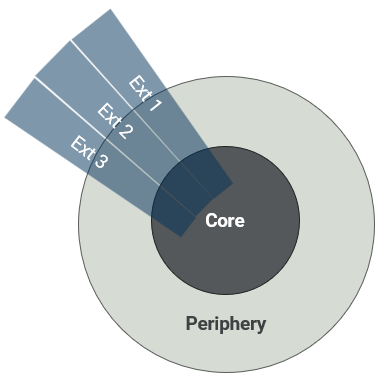
\includegraphics[width=1\linewidth]{figures/Rings.png}
    \caption{Enter Caption}
    \label{fig:placeholder}
\end{figure}

Notably, all three rings ultimately distill down to entities, relationships, and attributes, regardless of where they fall. Necessary for the application of governance, they allow for recognition of the distinction between required and recommended (functionally the same in this model), versus optional, this serves to create the space for maturity keying and regulation-specific overlays later.

\subsection{The regulation-agnostic spine}\label{sec:spine}

The core was held to be strictly regulation-agnostic, with regulatory requirements addressed through a combination of abstraction, entity typing, and regulation-specific entities and relationships within extensions. When regulation profiles for the GDPR (European Union), CCPA/CPRA (California, United States), LGPD (Brazil), and DPDPA (India) were created, there was limited divergence from the core relationships. While there was the appearance of some semantic compatibility initially, these more reflected differences in the cultural and political framing of each regulatory regime rather than a genuinely different approach to encoding the operational reality of who is processing which data, for what purpose, under which legal authority. (TODO: Example here?) Ultimately, this was not dissimilar to the issues experienced earlier during entity-relationship mapping where two identical concepts had differing terminology under differing standards or regulations. Anecdotally, this close fidelity of core relationships transcending modern regulation likely draws its origins back to various canonical works in data privacy including the OECD Privacy Principles and the Fair Information Practice Principles (TODO: Cite these and add years for each parenthetically).

The data model is contemplated to contain (\texttt{ProcessingActivity}, \texttt{Purpose}, \texttt{PersonalDataCategory}, \texttt{LegalBasis}, and \texttt{PartyRoleInActivity}) that should appear in every conformant implementation, at every maturity level, under every supported profile. \texttt{ProcessingActivity} is the closest thing that could be reasonably called the "center" of the spine, with \texttt{Purpose} attaching through the processing-for-purpose relationship, \texttt{PersonalDataCategory} through processing-of-data, and \texttt{LegalBasis} attaching, at L3 maturity and above, through the \texttt{LegalBasisAssignment} reification so the assignment can carry its own dates and evidence. \texttt{PartyRoleInActivity} is itself a reification of role-in-activity, which is what permits the same party (legal entity) to hold different roles in different activities. This reflects, especially in large organizations, the increased prevalence of one legal entity routinely holding a role as a controller in one activity and a processor in another. This corrects a common normalization flaw where typing roles onto parties directly rather than onto their participation creates inaccuracy as to a party's role and thusly their specific obligations. It is recommended that a privacy program implementing the data model should establish these five classes first, regardless of which regulations drive its program.

In summary, privacy regulations are doing a lot of the same things in sometimes different words. Reading any single regulation suggests that everything it names is required structure, but comparison across regimes shows that regulations bundle their requirements with regime-specific field names, templates, and enumerations. Even a reading of multiple regulations in a sitting may not make this initially apparent, due in part to the topic breadth of modern comprehensive privacy laws. This reconciliation, as well as the implicit concepts that regulations assume, such as organizations having their own structures and heirarches to organize and articulate their work, is what forms the spine of the data model.  

The choice to route the regime-specific portion to overlays (GDPR Article 30's mandatory record fields being the canonical example) is what lets the core hold at 34 entities and 65 relationships across all four profiles. This sustains the value proposition of a reference implementation for organizations holding at least two differing regulatory obligations. I contemplate the costs associated with implementing a common data model is offset as regulatory complexity increases, which is expected especially for large organizations.

\subsection{Normalization, Reification, and making Entities out of associations}\label{sec:reify}

A meaningful subset of the entity relationships cannot remain simple edges once they are tracked comprehensively (i.e. cross-subdomain, with all relationships reflected), because operational reality requires that they carry their own metadata. Exmaples may include which legal basis applied to which activity at what point in time, which role a party held when a consent event occurred, or what evidence was logged when. This reflects a truth of data engineering that edges do not carry data, only entities can. As a result, the model promotes twelve associations to first-class reified entity classes. These are \texttt{PartyRoleInActivity}, \texttt{LegalBasisAssignment}, \texttt{ConsentEvent}, \texttt{ClassificationAssignment}, \texttt{IdentityStateTransition}, \texttt{NoticeDelivery}, \texttt{Mitigation}, \texttt{Notification}, \texttt{SubmissionSnapshot}, \texttt{RoleFlipEvent}, \texttt{RightExerciseActivity}, and \texttt{EffectivenessReview}.

The pattern is consistent across all twelve. Each represents a fact about a relationship that the organization must be able to date, attribute, evidence, or version independently of the endpoints it connects. A \texttt{ConsentEvent} is a dated, attributable occurrence with a capture mechanism and a withdrawal path, not a bare ``data subject consents to purpose'' edge. A \texttt{SubmissionSnapshot} freezes a defensible record of exactly what was filed and when. A \texttt{RoleFlipEvent} captures the a party's controller/processor posture changes for an activity the moment it occurs, which is also representative of the kind of transition that is commonly subject to regulatory scrutiny and fault (that also happens to be erased when working with edges). The DPV does acknowledge this underlying need but treats such promotion-to-node actions as a workaround (see gap #6 as this is related). The data model treats these as foundational implementation patterns, because every relationship requiring versioning, evidence, temporal validity, or attribution requires it. Building on this, data architectures targeting L3 or above maturity should implement these as first-class entities from the start, because designs that leave them as edges force a large rework at L4 with significant cost overheads observed in maturity analysis (Section~\ref{sec:maturity}).

\subsection{Stuff without a clear home}\label{sec:crosscut}

Several things observed in widespread usage, "things" used in an ontological sense, simply don't sit cleanly in any single capability subdomain. Instead appearing across many in subtly different forms. Documents and assessments produced for accountability, transparency, and risk purposes serve cross-subdomain functions but are physically generated within whichever subdomain triggered them, so per-subdomain analysis renders each occurrence as a local entity. Only the cross-subdomain view typically pinpoints the shared parent. Ultimately, three unifying classes emerged from more detailed examination of this issue. \texttt{AccountabilityArtefact} is the abstract parent of 23 typed document subtypes spanning data processing agreements, joint-controller arrangements, sub-processor authorizations, and consent records, among others. \texttt{Notice} is a thin abstract parent whose concrete subtypes are co-owned by the subdomain triggering their issuance. (TODO: make this sentence a little less abstract) \texttt{ImpactAssessment} is polymorphic over the DPIA, PIA, FRIA, and TIA variants. Modeling these as shared parents rather than parallel local structures prevents drift between equivalent subtypes, reduces redundant fields, and centralizes the audit and retention logic that would otherwise be replicated across subdomains. It also reflects a practical reality that large organizations assess activities broadly across geographic boundaries and abstractions of harm types (e.g. harms to the organization, individuals, and society). 

\subsection{Connecting subdomains}\label{sec:joins}

The 87 cross-subdomain joins cataloged in the model exist because forced interoperability was a defining design constraint. Each subdomain produces or consumes structure that other subdomains need, and the join inventory is the basis on which inter-subdomain consistency can be planned. Beyond being informative, this also enables monitoring use cases associated with higher maturity levels, mitigating the need to "rediscover" a change every time a subdomain is touched. Expanding on maturity, these joins play a key role in enabling the maturity keying features (Section~\ref{sec:maturity}) of the data model because joins require compatible structures on each endpoint. Entities, Roles \& Accountability participates in 23 joins, the most of any subdomain, consistent with its role as the model's accountability backbone and the place where all obligations must pass through on query (Table~\ref{tab:subdomains}).

\subsection{Accounting for regulation}\label{sec:regulation}

Regulation attaches to the spine as profiles. Profiles can be conceptually visualized as overlays. They specifically add mandatory concepts not otherwise addressed through a regulation-agnostic approach as entities and relationships, and occasionally attributes or types. Four full profiles (GDPR, CCPA/CPRA, LGPD, DPDPA) and a small set of sectoral skeletons (e.g., HIPAA, GLBA) were composed for this exercise. The design consequence is that operating under multiple regulations more closely resembles a composition problem than a reconciliation one. Because no regulation scheme is reflected in the core, multi-regime processing is supported by implementing the core data model and selecting the appropriate overlays. This has the somewhat intended byproduct of surfacing conflicts for explicit assessment, handling, and decision, rather than being latent.

Consider a SaaS provider operating in both the United States and the European Union, with a single product-analytics processing activity touching personal data of California and EU residents. Under composition, the activity exists once in the core, with one \texttt{ProcessingActivity}, one set of \texttt{Purpose} and \texttt{PersonalDataCategory} attachments, and one \texttt{PartyRoleInActivity} arrangement. The GDPR profile then overlays the Article 30 record fields, the lawful-basis constraint, and the EU-specific transfer mechanic. The CCPA/CPRA profile overlays its disclosure categories, the sale/share flags, and its opt-out semantics. The union composes without error or conflict because the overlays touch different attributes, and where the regulatory schemes do genuinely diverge (e.g. retention expectations) the divergence surfaces as an explicit decision on the composed record. Under reconciliation, by contrast, the organization must classify the activity as ``a GDPR record'' or ``a CCPA record'' and then bolt the other regime on as an exception, which is a commonly observed pattern in most commercial tooling today.

This reflects an intentional design decision where target organizations operate across multiple jurisdictions and may enter new ones. Bypassing the regulation-agnostic core for short-term convenience produces the regime-coupling problem the model exists to prevent. This further supports the idea that organizations with cross-jurisdictional processing should accordingly resist process designs and/or tools that demand a single regulatory classification per processing activity. 

\subsection{Accounting for growth and maturity increase}\label{sec:maturity}

As large organizations seek to understand and control their privacy risk, they will likely desire to improve the process maturity within certain areas to provide assurance on privacy-relevant information and privacy controls. However, complex features (versioning, immutability of histories, temporal validity, edge provenance, and attestation) introduce unnecessary complexity at the lowest maturity levels that could threaten early and successful adoption. The model therefore contemplates these features separately, introducing them as between L3 and L5 that focuses on minimizing rework. Organizations that advance their maturity should expect to add these features to their clean core, and the model makes the cost of doing so explicit through 84 cataloged rework points across the twelve subdomains (Table~\ref{tab:rework}). It should be noted that a key finding here is the uneven distribution of rework points, with L3$\to$L4 as the cliff. This is mostly attributable to reification-validity semantics, the requirement that key associations carry versioning, temporal validity, and provenance. 

\begin{table}[ht]
\centering
\caption{Rework points by CMMI transition, with the character of each transition.}
\label{tab:rework}
\small
\begin{tabular}{@{}l l r@{}}
\hline
Transition & Character & Rework points \\
\hline
L1$\to$L2 & Register existence & 13 \\
L2$\to$L3 & Spine assembly & 14 \\
L3$\to$L4 & Reification cliff & 44 \\
L4$\to$L5 & Automation & 13 \\
\hline
Total & & 84 \\
\hline
\end{tabular}
\end{table}

Each transition has a distinct character. L1$\to$L2 is essentially \emph{register existence}, where the subdomain's primary records come into being as maintained data at all, and the rework is uniformly low because there is little structure, no enforcement on that strufture, and limited contemplation of entity-to-entity relationships. L2$\to$L3 is \emph{spine assembly}, where local records connect to the shared core classes, terminology begins to align to a common vocabulary, and consideration for cross-subdomain relationships begin but are still tolerant for duplication through low normalization. L3$\to$L4 is the \emph{reification cliff}, showcasing more than half of the rework points because structures that existed as simple records and edges at L3 must be retrofitted to carry history, validity intervals, and provenance. L4$\to$L5 is \emph{automation rather than new structure}, where the data model largely stops changing and the rework concerns instrumentation, monitoring hooks, and the closing of feedback loops. An organization budgeting a program, "budgeting" here in a broad and not purely financial sense, can read its costs casually off this profile. An L3$\to$L4 plan that funds process change and training without provisioning for time, funding, and technology to handle the versioned schemas and immutable event logs has ultimately underprovisioned the initiative, and it seems plausible to me that this is the next most common reason such initiatives stall.

In another dimension of change, it is also important to recognize that progress is often not free. The model documents 36 cross-subdomain dependencies, where certain maturity improvements presuppose that adjacent subdomains are already operating at a minimum (i.e. change-compatible) level. If they are not, the dependent subdomain simply will not accept the data model change as a function of incompatibility. Entities, Roles \& Accountability is the most depended-upon subdomain (7 inbound dependencies), followed by Legal Basis Management (6), which identifies these two as the highest-return early investments. Regulatory Reporting \& Disclosure, by contrast, is downstream of nearly everything, consistent with the principle that a report should be a view over the inventories rather than hand-kept primary data. Together, the rework points and the dependency map allow investment to be articulated and planned against a delta map, rather than reverse-engineered from known past program deficiencies. This is one of the model's headline practitioner utilities, making the costs of getting better estimable in advance by a mechanism of better forward view.

A final condition observed was the potential cost of operating at mixed maturity levels, which most organizations do in practice. Cross-subdomain joins require a degree of symmetry between their endpoints. When one side of a join operates at L4 and the other at L3, the L4 side must either degrade to L3 semantics across that join or use translation logic. Functionally, reification-validity semantics do not degrade gracefully, making translation approaches difficult in practice and leading to second-order effects such as losing provenance. This could force re-derivation (i.e. backsliding), which should be viewed as a kind of fault when it occurs. Functionally, this would be expected to occur during evolutions such as system migrations, M\&A integrations, and legacy decommissions and should be flagged as risks to the program's maturity and its data integrity, rather than being absorbed as IT work. Practically, an approach where level parity within connected clusters of subdomains is indicated, especially over maximizing any single subdomain in isolation. Per-subdomain rework and dependency figures appear in Table~\ref{tab:subdomains}. The full transition-level rework distribution and the pairwise dependency matrix appear in Appendix E.(TODO: Add link). 

\subsection{Accounting for and expressing risk tolerance}\label{sec:risk}

Certain entities and relationships appear in neither the clean core nor any regulation or maturity overlay. These are discretionary at the lowest maturity levels although they do become the source of dependency as maturity increases in both their own and adjacent domains. As a matter of technical correctness, imposing them as mandatory from the outset of implementation would be arbitrary and resolving them in the model would impose a single risk posture on every adopting organization. That said, they are likely happening in large organizations already and there may also be reasons for their implementations beyond risk tolerance such as staff efficiency or for enabling monitoring in an adjacent subdomain. Ultimately, forty of these points, represented as implementation decisions, were identified and made explicit, each documented with its options and trade-offs, and the full catalog is browsable in the model explorer (Section~\ref{sec:artifact}). (TODO: Add this to an appendix, then add a link, replacing the model explorer reference).

Beyond entities and relationships, the work surfaced the importance of implicit taxonomies and taxonomy-like typing schemes in the design of and within certain attributes. This is fundamentally expressed in degrees of coarseness, where the finer-tuned the individual taxonomy, the more precisely risk is expressed. This contemplates that intentionally applied precision serves as an expression of risk tolerance within that area. A universally applicable example is the precision an organization uses to describe the unit types of personal data. The choice carries no inherent entity relationship, but an organization that believes it can describe all possible types of personal data in 30 options versus 100 versus 300 is inherently accepting risk through its apparent precision or lack thereof. A hospital may need to represent dozens of medical-specific personal data attributes because of the varied sensitivity and abuse cases associated with diagnosis information differ from those of a common test result such as an EKG. Further, a food manufacturer may reasonably compress this same information under the single umbrella of ``Medical Records''. Coarseness need not be uniformly applied though and these specific decisions remain a a valuable lever for an organization to articulate its risk tolerance as part of the construction of its due diligence processes. This also reflects a practical reality that organizations must establish processes before they monitor them.

The same pattern recurs at larger scales. Orienting the risk taxonomy on harms, rights, or impacts is a defensible choice in every direction, with each orientation represented among the authoritative sources, and the choice propagates into assessment templates, mitigation typing, and regulator-facing narratives. Whether the four control themes inherited from ISO/IEC 27002 (TODO: add a citation) (technical, organizational, legal, physical) are modeled as a class hierarchy or an attribute facet has no correct answer in the abstract, but it carries material consequences for how controls are queried, inherited, and reported once thousands of instances exist. 

Similarly, adopting a CMMI target of L2 versus L4 in a process subdomain is itself a manifestation of risk tolerance. However, it was observed that opportunity for discretion narrows as maturity rises. This is attributable to the many decisions that are defensible either-way at L2 collapsing toward a single valid resolution once versioning and provenance requirements are implemented between L3, L4, and L5. This creates an imperative for organizations approaching a transition to resolve the relevant decisions before continuing. 

Lastly, the relationship between large organizations and commercial tool providers must be confronted at this stage. The analysis also included an inspection of input taxonomies implemented by commercial tool providers, namely, the API schemas that reflect, to some degree, the design of their product's own data models. 

While I previously asserted that these decision points had no single correct answer, the degree to which commercial tool providers 1) recognize these as decision points 2) subsequently recognize them as as dimensions to express risk tolerance for the implementing organization and 3) support customization and extension of these as features widely vary across the corpus of commercial privacy tools. This dynamic should create a few imperatives for organizations to ensure that any commercial tools they choose to employ will support appropriate extensibility based on their maturity requirements and ambitions, especially when making build/buy decisions. 

In all cases, understanding where these decisions exist implicitly and taking steps to decision their design reflects an explicit choice to control risk with somewhat enumerated trade-offs, rather than implicit risk acceptance by default.

\subsection{What the model looks like in each program area}\label{sec:areas}

While the previous sections describe the various viewpoints and requirements that inform the model's design philosophy, this one walks through its functional mechanics. 
Table~\ref{tab:subdomains} summarizes the characteristics referenced throughout this walkthrough.

% TODO: reconcile the column sums below against the prose counts (34 core
% entities / 51 per-subdomain entities; 65 core / 37 per-subdomain
% relationships) -- the source tables and prose measure overlapping but
% distinct populations. Also note: transition-level rework rows in
% Appendix E Table 3 sum to 81 while the published totals row sums to 84;
% verify before camera-ready.
\begin{table*}[ht]
\centering
\caption{Per-subdomain characteristics of the reference model, covering local entities and relationships, cross-subdomain joins, total maturity rework points, and dependency counts. Outbound dependencies count the subdomains this one must wait for. Inbound dependencies count the subdomains waiting on this one.}
\label{tab:subdomains}
\small
\begin{tabular}{@{}l r r r r r r@{}}
\hline
Subdomain & Entities & Relationships & Joins & Rework & Dep.\ (out) & Dep.\ (in) \\
\hline
1 -- Processing Inventory & 2 & 20 & 17 & 6 & 6 & 4 \\
2 -- Purpose Specification \& Governance & 2 & 5 & 6 & 4 & 5 & 2 \\
3 -- Personal Data Inventory \& Classification & 7 & 14 & 7 & 6 & 1 & 4 \\
4 -- Legal Basis Management & 5 & 8 & 16 & 8 & 4 & 6 \\
5 -- Entities, Roles \& Accountability & 12 & 30 & 23 & 9 & 1 & 7 \\
6 -- Consent Management & 4 & 10 & 9 & 6 & 3 & 2 \\
7 -- Data Subject Rights Management & 5 & 9 & 5 & 6 & 3 & 1 \\
8 -- Notice \& Transparency & 5 & 4 & 6 & 7 & 0 & 1 \\
9 -- Risk \& Impact Assessment & 3 & 8 & 12 & 10 & 3 & 4 \\
10 -- Technical \& Organizational Measures & 4 & 9 & 7 & 8 & 1 & 1 \\
11 -- Incident \& Breach Management & 5 & 9 & 10 & 6 & 4 & 2 \\
12 -- Regulatory Reporting \& Disclosure & 5 & 3 & 5 & 5 & 5 & 2 \\
\hline
\end{tabular}
\end{table*}

Of the twelve subdomains, these can further be grouped into four clusters that further illustrate function, purpose, and distribution of entities and relationships.

Subdomains 1 through 5 (Processing Inventory, Purpose Specification \& Governance, Personal Data Inventory \& Classification, Legal Basis Management, and Entities, Roles \& Accountability) together constitute the processing spine, and their shapes are instructive. Processing Inventory carries only 2 entities but 20 relationships and 17 cross-subdomain joins. It is a hub of interconnection that contains the context of organizational activities. Entities, Roles \& Accountability is the model's largest subdomain by every measure (12 entities, 30 relationships, 23 joins), consistent with its role as the accountability checking mechanism and its position as the most depended-upon subdomain in the maturity dependency map. Legal Basis Management is compact locally (5 entities, 8 relationships) but joins broadly (16), reflecting that lawful basis is asserted \emph{about} other subdomains' records rather than existing for its own sake. Personal Data Inventory \& Classification carries the model's densest attribute typing, because it is where the unit-of-accounting and classification-scheme decisions of Section~\ref{sec:risk} land.

Subdomains 6 through 8 (Consent Management, Data Subject Rights Management, and Notice \& Transparency) are best characterized together as individual facing operations, these share a common thread of event-focused reification-dependent structures tightly coupled to the data subject's point of view. Consent Management is built around the \texttt{ConsentEvent} reification and its withdrawal path. Rights Management is built around \texttt{RightExerciseActivity} and its time-sensitive workflow states. Notice \& Transparency is built around \texttt{NoticeDelivery}, which converts ``we published a notice'' into ``this notice version reached this audience through this mechanism at this time.'' Despite being among the most visible obligations in privacy law, it has one of the thinnest subdomains (4 local relationships, the fewest in the model). This is because of the inherent relationship between notice and consent, where consent is often given pursuant to the specific terms of a notice. This "light" structure is not dissimilar from entities that exist primarily to summarize and present information mastered elsewhere such as \texttt{AccountabilityArtefact}.

Subdomains 9 through 11 (Risk \& Impact Assessment, Technical \& Organizational Measures, and Incident \& Breach Management) form the program's risk and controls cluster. Risk \& Impact Assessment is compact (3 entities) but carries the model's highest rework total (10 points), because these assessments accumulate the most L4 changes that introduce detail necessary to more precisely assess risk. They also include versioned findings, \texttt{Mitigation} reifications, and \texttt{EffectivenessReview} support. It also joins broadly (12), because an assessment is fundamentally a claim about other subdomains' records. Technical \& Organizational Measures hosts the control-theme decision discussed in Section~\ref{sec:risk} and links the privacy program to the wider security control estate through loosely adherant NIST OSCAL-style structures~\cite{nistoscal}. Incident \& Breach Management is where the \texttt{Notification} reification exists to bridge gaps between the organization, individual regulations, and individual breach obligations. Notification obligations extend per-regulation and per-authority. This is intentional and in contrast to the prevailing common approach that has notification modeled as an attribute of the incident. By doing this, it allows demonstration of timeliness of meeting notification requirements, which is a frequently enforced obligation within this subdomain.

Regulatory Reporting \& Disclosure, subdomain 12, is deliberately the thinnest in local structure (3 local relationships) and among the most dependent in the map (5 outbound dependencies). This is a design position that considers the reports and disclosures made in this subdomain should be a view of the inventories, materialized through \texttt{SubmissionSnapshot} records for defensibility, and never primary hand-kept data. Maintaining a regulator-facing report as primary data is a maturity anti-pattern the model will not enable. The corollary, captured in the dependency map, is that this subdomain cannot reach L4 until many of its respective source inventories have.

\subsection{Defining boundaries between the DPV and reference model, considering DPV gaps}\label{sec:boundary}

The boundary between the DPV's appropriate ontological scope and the reference-model's definition is an analytic result of this work. The DPV publishes concept schemes while the reference data model contemplates something that resembles a schema. Where an organization depends on regulation, maturity, or risk tolerance, it likely belongs within the reference model or below. community had already opened adjacent discussion.

Against that boundary, the reference data model build identified 13 specific gaps in the DPV, of which at least three were previously undocumented. Ten of thirteen are substantively improved upon within this work.

The largest gaps concerned maintenance and freshness mechanics. Regulations and standards uniformly require records to be ``kept up to date'' while giving little guidance on how or freshness expectations. Across the entire input corpus, no surveyed taxonomy provided the mechanism to operationalize the requirement, leaving every adopting organization to originate the same structure independently. The reference data model closes this gap directly, originating a maintenance-status state machine supported by a freshness triad (last-reviewed timestamp, review cadence, and next-review-due) together with attestation and reviewer-identity attributes. The mechanism is introduced at L3, enforced at L4, and automated at L5, and it applies uniformly across the inventory and assessment subdomains. Retrofitting freshness metadata after the fact is among the most expensive periphery additions in the rework catalog. It is recommended that the freshness mechanism be adopted into every inventory and assessment at L3, even where the review processes it supports are not yet formalized.

\subsection{The delivered artifact}\label{sec:artifact}

The model is delivered in two coordinated forms. 

\begin{enumerate}
    \item Machine-readable schema, a hybrid OWL/RDFS ontology in Turtle (.ttl) format of approximately 1,200 lines, compatible with common ontological tools such as Prot\'eg\'e. Available at (TODO: Insert)
    \item the interactive Reference Data Model Explorer web application, available at \texttt{PrivacyReferenceModel.com}, which exists because the model's breadth does not present neatly on a single diagram. The explorer supports graph visualization with target-maturity filtering (which reduces complexity to the selected level), layer isolation across core, periphery, and profile extensions, and standalone catalogs for subdomains, entities, relationships, decisions, and maturity levels. 
\end{enumerate}

A third form is contemplated but was not delivered as part of this work. This will be an implementation guide that will include a documentation set, including the per-subdomain models with individual visualizations along with the decision and maturity-delta catalogs. This is further discussed in Section~\ref{sec:lqfw}.

% Figure skeletons for the explorer screenshots (currently Appendix A).
% Uncomment and point at your image files:
% \begin{figure}[ht]
%   \centering
%   \includegraphics[width=\linewidth]{figures/explorer-graph.png}
%   \caption{The Reference Data Model Explorer graph view, filtered to a
%     target maturity level with core, periphery, and profile-extension
%     layers isolated.}
%   \label{fig:explorer-graph}
% \end{figure}
%
% \begin{figure}[ht]
%   \centering
%   \includegraphics[width=\linewidth]{figures/explorer-detail.png}
%   \caption{Entity detail pane showing related entities, relationships,
%     and metadata for a selected class.}
%   \label{fig:explorer-detail}
% \end{figure}
\textbf{TODO:} insert explorer screenshots (figure skeletons provided in comments).

\section{Limitations, Qualifications, and Future Work}\label{sec:lqfw}

\subsection{Limitations}\label{sec:limitations}

Several limitations bound this work. First, the Technology \& AI Governance subdomain was deliberately set aside because its regulatory environment and position within the DPV is still stabilizing (TODO: Add DPV citation). While there is no absence of available input taxonomies in the space, many lack detail to support modeling depth and it is not yet clear which will end up with high levels of authority, ultimately substituting speculation for evidence.

Second, the internal validity evaluation, while systematic, stops short of synthetic-data stress testing. The 100 test cases validate satisfiability of the model's structure, not performance or behavior under realistic data volumes. 

Third, external validity is the weakest part of the work to date. The W3C working group does not typically comment on individual implementations, feedback on the submitted issues remains pending, and broader qualitative validation would require a high degree of screening on feedback subjects in a topic this specialized, an effort that exceeded the available time and effort.

Finally, the maturity grounding is CMMI-esque at best and should not be taken as a strict implementation. The maturity-delta, including its concentration cliff between L3 and L4, is likely a manifestation that there may be a more fit for use mechanism to express the intersection of process maturity requirements, risk tolerance, and required data. If restarting with this knowledge, the work could be made more concrete by abstracting CMMI and defining a single level of required minimum normalization per CMMI level starting with sixth normal form (6NF) or domain-key normal form (DKNF) for CMMI Level 5 as an application of  and then working downwards from there. This would add a certain level of concreteness to the data structure model at each maturity level.

(TODO: Go back and cite CMMI for Services)

applying the continuous representation in spirit rather than as a strict assessment of requirements of CMMI  mapping to CMMI practice areas. This is not a fully faithful cross-mapping against CMMI and on a re-do, I'd slightly modify the approach to examine data

\subsection{Qualifications}\label{sec:qualifications}

The claims of this work should be read under several qualifications. This is a reference model, not a standard. It carries no conformance authority, and the idea of a ``perfect'' data model is not that implementing organizations can be perfect, but that the model is a rigorous starting point from which implementers decide what is good enough for their organizations based on their own context. The published counts are a versioned snapshot against DPV 2.3 and the cited regulatory texts as of this writing. Source traceability guarantees provenance, not correctness. The input taxonomies themselves may err, and where they disagree, this work's resolutions are documented judgments rather than discovered facts. Applicability assumes the DPV framing and a CMMI-style maturity lens, and the model is oriented toward large, multi-jurisdictional organizations, so smaller or single-regime organizations may find portions of the periphery permanently out of scope.

The work should also be read against the adjacent efforts it does not replace. Commercial platforms embody the most complete privacy data models in practical existence, observable through their public API surfaces~\cite{bigid_api_overview, datagrail_api_v2_reference, onetrust_api_reference, securiti_api_reference, trustarc_gateway_api_developers_guide}, but they are implicit, proprietary, and shaped by the vendor's need to satisfy a diverse customer base, and this work has not been evaluated against them directly. Academic privacy engineering work, including privacy-by-design (TODO: Cite kevoukian) methodology~\cite{cronkspbd} and threat-modeling frameworks such as LINDDUN~\cite{linddun}, addresses how to analyze and design for privacy rather than what the operating data structures must be, and this model does not substitute for either. To my knowledge, no prior work has attempted a full-breadth, maturity-parameterized, regulation-agnostic reference data model for organizational privacy operations with the DPV as its semantic foundation. That novelty cuts both ways, because it also means no independent benchmark exists to compare the composed whole against, and this absence is part of why external validity remains the weakest pillar and such a large task to evaluate.

\subsection{Future Work}\label{sec:futurework}

I contemplate that there are at least five areas for future work, building on this:

\begin{enumerate}
    \item A full implementation guide should accompany the reference model, translating its structures into adoption sequences for organizations at differing starting maturities.
    \item  Internal validity can be deepened through synthetic-data testing against the Turtle serialization. 
    \item External validity can be expanded through a screened expert panel and subsequent continuous feedback during organizational implementations once scoping burden can be supported.
    \item There is value in this work as a diagnostic framework to help organizations assess their privacy program maturity and readiness via their data. This channels questions that sound like \emph{What (data) do you have today? What (tasks) could/should operationalize next? What domains could be operationalzied with relatively low cost?} and \emph{What is the corpus of privacy program tasks that needs to be performed?}
    \item There may b further diagnostic merit in using the model as an evaluation instrument against common commercial tools with the aim of pinpointing exactly what maturity level their implicit data structures imply, extend to, or max out at.
\end{enumerate}

\section{Conclusions}\label{sec:conclusion}

This work began from the observation that privacy compliance difficulty in large organizations resembles a convergence problem, where implementing regulatory guidance, independent standards, or commercial tools each produce mostly valid work in isolation, with organizations holding the bag of data trying to make it all work together compatibly under the auspices of a privacy program. 

Treating that failure as a data problem first, the work asked what a truly unified data model for privacy within a large organization would look like if interoperability across common process domains were forced. The methodology involved reconciliation of approximately 50  authoritative taxonomies against the W3C DPV into an implementable reference data model, subsequently evaluated through 100 machine-validated test cases.

Three conclusions carry beyond the artifact. A
(TODO: Come back to these) 

2. The importance of identifying and reserving latent decisions as a function of risk.
3.  the costs of getting better estimable in advance by a mechanism of better forward view.


vocabulary is not a schema. The structure required to operate a privacy program exceeds the DPV's published surface by an order of magnitude, and that structure will be committed somewhere, either through architectural deliberateness or implicitly by a commercial tool. The backbone that all regulations share is smaller than any one regulation implies, which is what makes a regulation-agnostic core with composable overlays achievable, and worth the investment for any organization holding two or more regulatory obligations. And once the model is parameterized by maturity and risk and every element is traceable to its source, the cost of getting better becomes estimable, with rework points, dependencies, and decision points converting maturity advancement from a discovered expense into a planned one.

There is also a lesson here beyond privacy. Ontologies, taxonomies, and reference schemas exist for a whole host of domains, including incident response, vulnerability management, and identity, and the approach demonstrated here generalizes. Ideate on what the data would look like if the problem no longer existed, work backward from that, and watch the places where you do not control your own data structures. If you want to get better at something, endeavor to be more precise. That mindset applies to data through normalization, and the quality of any AI system is bounded by the quality of the semantic structures beneath it. Garbage in, garbage out will always prevail. The remaining question is the one this model can price but not answer for you. When is it time to do the work, rather than accept the status quo as a buy-versus-build decision?


\section*{Acknowledgments}
\subsection*{GitHub Repository}
    Visit the repository to access the source code, track ongoing development, report issues, and stay up to date with the latest changes.
    \begin{center}
        \setlength{\tabcolsep}{3pt}
        \begin{tabular}{cl}
             \faGithub &  \url{https://github.com/bricedobson/Privacy-Taxonomy}\\
        \end{tabular}
    \end{center}
\subsection*{Thanks}
The author would like to thank the following individuals and groups for their influence on this work. 
\begin{itemize}
    \item Dr keurbis and Emad.
    \item The W3C Working Group
    \item the paper 'how to write papers'
    \item ontology book guy, amateur ontologist.
\end{itemize}
\subsection*{AI Use Disclosures}
Generative AI was used in the completion of this work in the following ways.
\begin{itemize}
    \item Proofreading and associated editing for style, clarity, and brevity within this report.
    \item Conversion of source metadata to BibTeX format.
    \item Formatting support with \LaTeX and BibTeX
    \item Transformation of raw analysis files to a properly formatted RDF OWL Hybrid Ontology file and associated debugging.
    \item Transforming the analysis schema to a format compatible with the web-based explorer.
    \item Various code implementations and improvements within the web-based explorer application.
\end{itemize}
\subsection*{Template}
 This document was compiled using \href{https://github.com/MemoJimenez/Rho-class}{Rho-class}, a \LaTeX{} template developed by Guillermo Jimenez.
 \clearpage
\onecolumn
%\appendix
\section{Appendices}
\subsection{Appendix A: Full Data Model}
\label{sec:a}
\begin{center}
    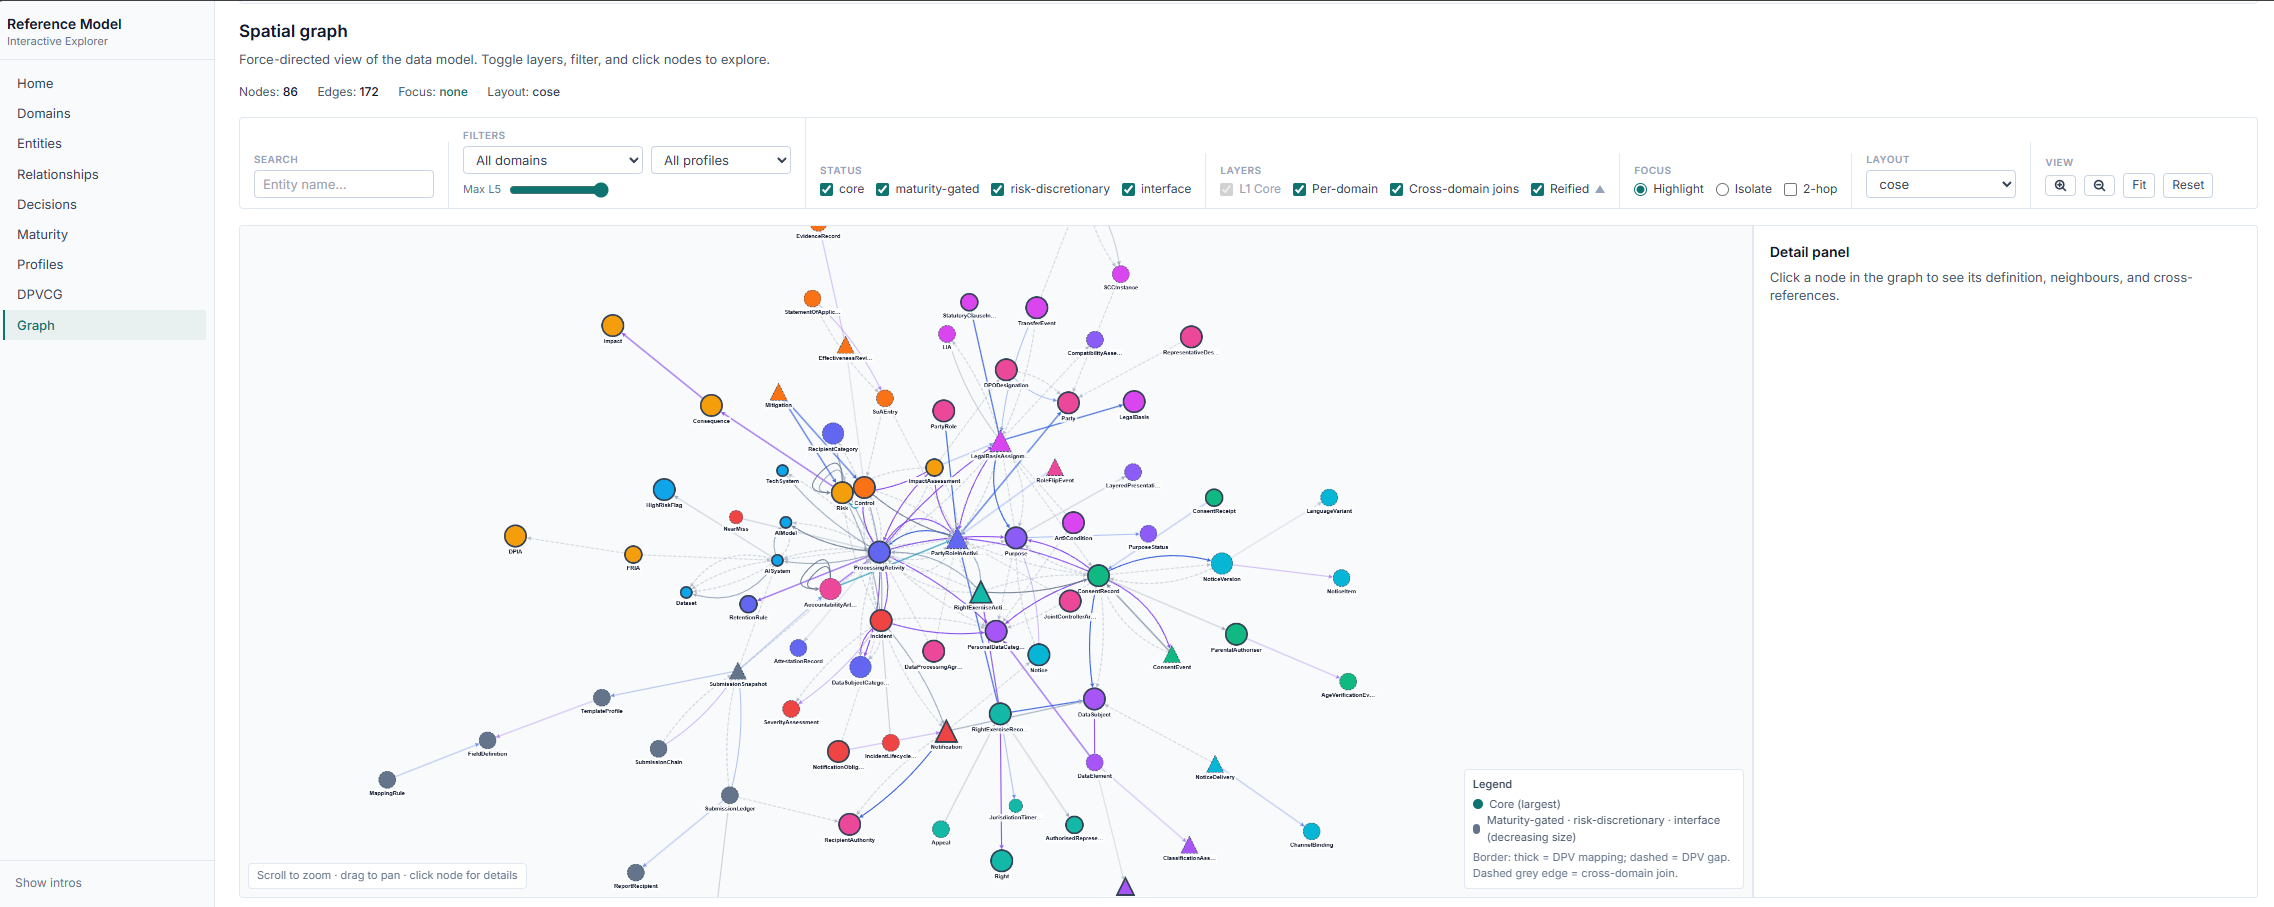
\includegraphics[width=.9\linewidth]{figures/Temp.png}
    \captionof{figure}{Placeholder Screenshot for Progress Report of Data Model within Explorer App}
\end{center}

\vspace{1em}

\begin{center}
    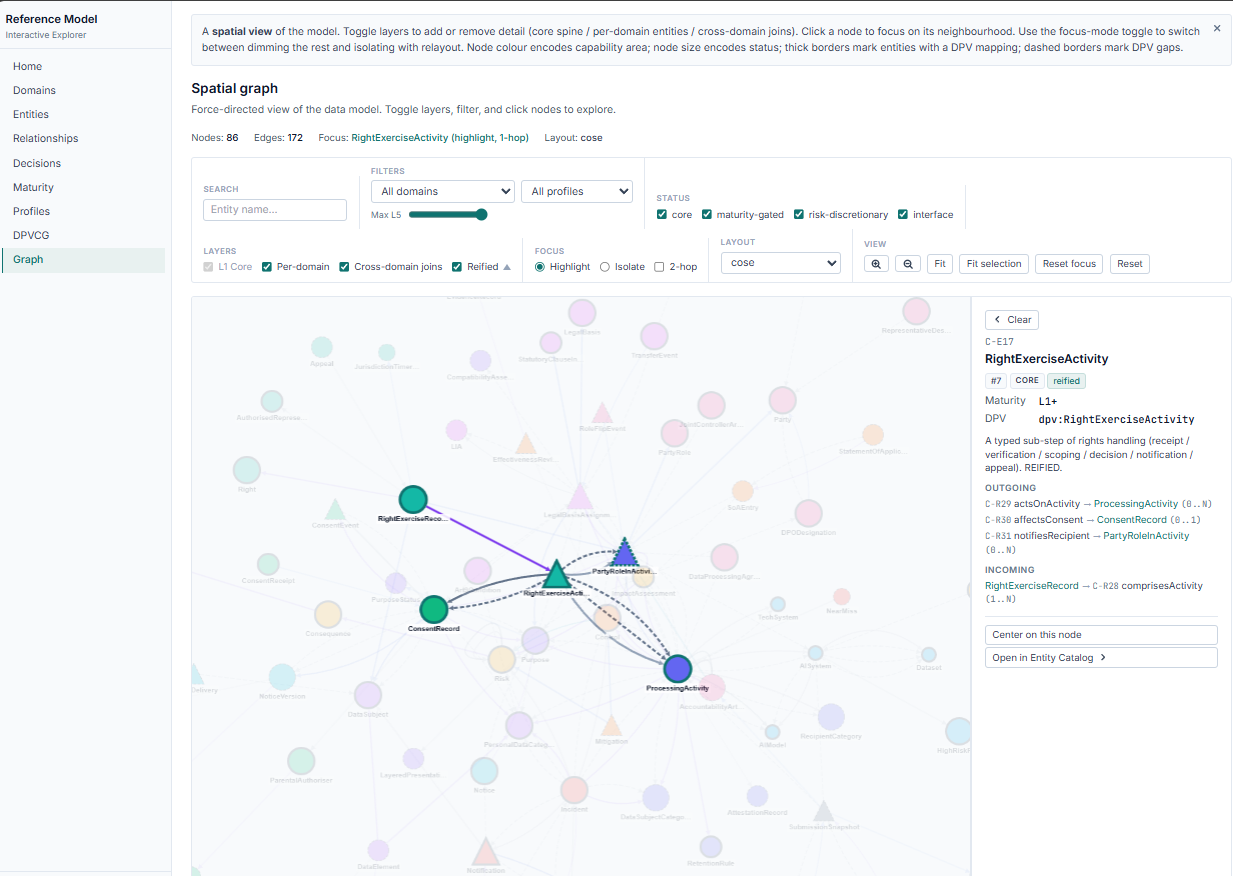
\includegraphics[width=.9\linewidth]{figures/image.png}
    \captionof{figure}{Additional example showcasing the detail pane on selection of a specific entity}
\end{center}

\clearpage
\subsection{Appendix B: Full Listing of Input Taxonomies by Author Type Classification}
\label{sec:b}
\subsection{Appendix B: Full Listing of Input Taxonomies by Author Type Classification}
\label{sec:b}
\subsubsection*{Independent Standards}
\printbibliography[heading=none,filter=taxonomystandards]
\subsubsection*{Governmental}
\printbibliography[heading=none,filter=taxonomyregulatory]
\subsubsection*{Commercial}
\printbibliography[heading=none,filter=taxonomycommercialtools]
\subsubsection*{Academic Work}
\printbibliography[heading=none,filter=taxonomyacademicwork]
\clearpage
\subsection{Appendix C: Mapping of Taxonomies to Domains}
\begin{longtable}{@{}p{0.28\linewidth} p{0.68\linewidth}@{}}
\caption{Input taxonomies mapped to the twelve capability-area domains of the reference model, based on the DPV.\\ \textbf{TODO:} Fix the numbering issue with the references}%
\label{sec:c}\\
\toprule
\textbf{Capability-area domain} & \textbf{Input taxonomies}\\
\midrule
\endfirsthead
\multicolumn{2}{@{}l}{\textit{Table~\ref{tab:taxonomy-domain-map} (continued)}}\\
\toprule
\textbf{Sub-Domain Process Area} & \textbf{Input taxonomies}\\
\midrule
\endhead
\midrule
\multicolumn{2}{r@{}}{\textit{(continued on next page)}}\\
\endfoot
\bottomrule
\endlastfoot

\#1 Processing Inventory &
\cite{gdpr,dpv,iso27701,iso29100,iso15489,nistprivacyframework11ipd,cnilropa,dpcat,ccpacpra,bigid_api_overview,onetrust_api_reference,securiti_api_reference,trustarc_gateway_api_developers_guide}\\
\addlinespace

\#2 Purpose Specification \& Governance &
\cite{gdpr,dpv,wp203,iso19944part1,iso19944part2,iabtcf,ccpacpra,pipl,onetrust_api_reference,trustarc_gateway_api_developers_guide}\\
\addlinespace

\#3 Personal Data Inventory \& Classification &
\cite{gdpr,dpv,iso29100,iso19944part1,iso19944part2,nistprivacyframework11ipd,enterprivacycategories,cronkspbd,ccpacpra,lgpd,pipl,bigid_api_overview,onetrust_api_reference,securiti_api_reference}\\
\addlinespace

\#4 Legal Basis Management &
\cite{gdpr,dpv,iso27701,ccpacpra,lgpd,pipl,onetrust_api_reference,trustarc_gateway_api_developers_guide}\\
\addlinespace

\#5 Entities, Roles \& Accountability &
\cite{gdpr,dpv,iso27701,iso29100,ccpacpra,lgpd,pipl,dora,onetrust_api_reference,trustarc_gateway_api_developers_guide}\\
\addlinespace

\#6 Consent Management &
\cite{gdpr,dpv,iso27560,iso29184,kantaracr,ieee7012,iabtcf,gpc,adpc,eprivacydirective,dga,ccpacpra,datagrail_api_v2_reference,onetrust_api_reference,trustarc_gateway_api_developers_guide}\\
\addlinespace

\#7 Data Subject Rights Management &
\cite{gdpr,dpv,edpberasure2026,ccpacpra,lgpd,pipl,datagrail_api_v2_reference,onetrust_api_reference,securiti_api_reference,trustarc_gateway_api_developers_guide}\\
\addlinespace

\#8 Notice \& Transparency &
\cite{gdpr,dpv,wp260,iso29184,ieee7012,gpc,adpc,eprivacydirective,ccpacpra,onetrust_api_reference,trustarc_gateway_api_developers_guide}\\
\addlinespace

\#9 Risk \& Impact Assessment (DPIA/PIA) &
\cite{gdpr,dpv,iso27005,iso31000,nistir8062,nistpram,nistprivacyframework11ipd,linddun,cnilpia,cnilpiasoftware,icodpia,owaspprivacy,enisathreattaxonomy,onetrust_api_reference,trustarc_gateway_api_developers_guide}\\
\addlinespace

\#10 Technical \& Organisational Measures &
\cite{gdpr,dpv,iso27701,nistoscal,nistprivacyframework11ipd,enisanis2guidance,owaspprivacy,onetrust_api_reference,securiti_api_reference}\\
\addlinespace

\#11 Incident \& Breach Management &
\cite{gdpr,dpv,eprivacydirective,dga,dora,doraits302,nistprivacyframework11ipd,enisathreattaxonomy,enisanis2guidance,nis2templates,onetrust_api_reference}\\
\addlinespace

\#12 Regulatory Reporting \& Disclosure &
\cite{gdpr,dpv,dpcat,nistoscal,cnilropa,doraits302,nis2templates,dora,dga,onetrust_api_reference,trustarc_gateway_api_developers_guide}\\

\end{longtable}

\clearpage
\subsection*{Appendix D: Taxonomy Extracted Data Relationships by Domain}
\clearpage
\subsection*{Appendix E: Summary Analysis Statistics}

\begin{small}
\setlength{\tabcolsep}{4pt}
\renewcommand{\arraystretch}{1.15}

\begin{longtable}{p{0.39\textwidth}ccccc}
\caption{Referemce Data Model Characteristics}
\label{tab:domain-inventory} \\

\hline
\textbf{Subdomain} &
\textbf{Entities} &
\textbf{Relationships} &
\textbf{Cross-Domain} &
\textbf{Decisions} &
\textbf{Rework Points} \\
\hline
\endfirsthead

\hline
\textbf{Domain} &
\textbf{Entities} &
\textbf{Relationships} &
\textbf{Cross-Domain} &
\textbf{Decisions} &
\textbf{Rework Points} \\
\hline
\endhead

\hline
\endfoot

\hline
\endlastfoot

\textbf{1 -- Processing Inventory} & 2 & 20 & 17 & 7 & 3 \\
\textbf{2 -- Purpose Specification \& Governance} & 2 & 5 & 6 & 3 & 1 \\
\textbf{3 -- Personal Data Inventory \& Classification} & 7 & 14 & 7 & 6 & 3 \\
\textbf{4 -- Legal Basis Management} & 5 & 8 & 16 & 2 & 5 \\
\textbf{5 -- Entities, Roles, \& Accountability} & 12 & 30 & 23 & 6 & 6 \\
\textbf{6 -- Consent Management} & 4 & 10 & 9 & 5 & 3 \\
\textbf{7 -- Data Subject Rights Management} & 5 & 9 & 5 & 6 & 3 \\
\textbf{8 -- Notice \& Transparency} & 5 & 4 & 6 & 2 & 6 \\
\textbf{9 -- Risk \& Impact Assessment} & 3 & 8 & 12 & 4 & 9 \\
\textbf{10 -- Control Measures} & 4 & 9 & 7 & 4 & 6 \\
\textbf{11 -- Incident \& Breach Management} & 5 & 9 & 10 & 2 & 3 \\
\textbf{12 -- Regulatory Reporting \& Disclosure} & 5 & 3 & 5 & 2 & 2 \\

\end{longtable}
\end{small}

\begin{small}
\setlength{\tabcolsep}{5pt}
\renewcommand{\arraystretch}{1.15}

\begin{longtable}{p{0.42\textwidth}ccccc}
\caption{Reference Data Model Rework Distribution}
\label{tab:reference-data-model-rework-distribution} \\

\hline
\textbf{Subdomain} &
\textbf{$L_1 \to L_2$} &
\textbf{$L_2 \to L_3$} &
\textbf{$L_3 \to L_4$} &
\textbf{$L_4 \to L_5$} &
\textbf{Totals} \\
\hline
\endfirsthead

\hline
\textbf{Domain} &
\textbf{$L_1 \to L_2$} &
\textbf{$L_2 \to L_3$} &
\textbf{$L_3 \to L_4$} &
\textbf{$L_4 \to L_5$} &
\textbf{Totals} \\
\hline
\endhead

\hline
\endfoot

\hline
\endlastfoot

\textbf{1 -- Processing Inventory} & 1 & 1 & 3 & 1 & \textbf{6} \\
\textbf{2 -- Purpose Specification \& Governance} & 1 & 1 & 1 & 1 & \textbf{4} \\
\textbf{3 -- Personal Data Inventory \& Classification} & 1 & 1 & 3 & 1 & \textbf{6} \\
\textbf{4 -- Legal Basis Management} & 1 & 1 & 5 & 1 & \textbf{8} \\
\textbf{5 -- Entities, Roles, \& Accountability} & 1 & 1 & 6 & 1 & \textbf{9} \\
\textbf{6 -- Consent Management} & 1 & 1 & 3 & 1 & \textbf{6} \\
\textbf{7 -- Data Subject Rights Management} & 1 & 1 & 3 & 1 & \textbf{6} \\
\textbf{8 -- Notice \& Transparency} & 1 & 1 & 4 & 1 & \textbf{7} \\
\textbf{9 -- Risk \& Impact Assessment} & 1 & 2 & 6 & 1 & \textbf{10} \\
\textbf{10 -- Control Measures} & 1 & 1 & 5 & 1 & \textbf{8} \\
\textbf{11 -- Incident \& Breach Management} & 1 & 1 & 3 & 1 & \textbf{6} \\
\textbf{12 -- Regulatory Reporting \& Disclosure} & 1 & 1 & 2 & 1 & \textbf{5} \\
\hline
\textbf{Totals} & \textbf{13} & \textbf{14} & \textbf{44} & \textbf{13} & \textbf{84} \\

\end{longtable}
\end{small}
\begin{scriptsize}
\setlength{\tabcolsep}{3pt}
\renewcommand{\arraystretch}{1.15}

\begin{longtable}{p{0.34\textwidth}ccccccccccccc}
\caption{Reference Data Model Dependency Map by Subdomain}
\label{tab:reference-data-model-dependency-map} \\

\hline
\textbf{Subdomain} &
\textbf{D1} &
\textbf{D2} &
\textbf{D3} &
\textbf{D4} &
\textbf{D5} &
\textbf{D6} &
\textbf{D7} &
\textbf{D8} &
\textbf{D9} &
\textbf{D10} &
\textbf{D11} &
\textbf{D12} &
\textbf{Total (Out)} \\
\hline
\endfirsthead

\hline
\textbf{Subdomain} &
\textbf{D1} &
\textbf{D2} &
\textbf{D3} &
\textbf{D4} &
\textbf{D5} &
\textbf{D6} &
\textbf{D7} &
\textbf{D8} &
\textbf{D9} &
\textbf{D10} &
\textbf{D11} &
\textbf{D12} &
\textbf{Total (Out)} \\
\hline
\endhead

\hline
\endfoot

\hline
\endlastfoot

\textbf{1 -- Processing Inventory} & 1 &  & 1 & 2 & 2 &  &  &  &  &  &  &  & \textbf{6} \\
\textbf{2 -- Purpose Specification \& Governance} & 1 & 1 &  & 2 &  &  &  &  & 1 &  &  &  & \textbf{5} \\
\textbf{3 -- Personal Data Inventory \& Classification} &  &  & 1 &  &  &  &  &  &  &  &  &  & \textbf{1} \\
\textbf{4 -- Legal Basis Management} &  &  &  & 1 & 2 &  &  &  & 1 &  &  &  & \textbf{4} \\
\textbf{5 -- Entities, Roles, \& Accountability} &  &  &  &  & 1 &  &  &  &  &  &  &  & \textbf{1} \\
\textbf{6 -- Consent Management} &  & 1 &  &  &  & 1 &  & 1 &  &  &  &  & \textbf{3} \\
\textbf{7 -- Data Subject Rights Management} &  &  & 1 &  &  & 1 & 1 &  &  &  &  &  & \textbf{3} \\
\textbf{8 -- Notice \& Transparency} &  &  &  &  &  &  &  &  &  &  &  &  & \textbf{0} \\
\textbf{9 -- Risk \& Impact Assessment} &  &  &  &  & 1 &  &  &  & 1 &  & 1 &  & \textbf{3} \\
\textbf{10 -- Control Measures} &  &  &  &  &  &  &  &  &  & 1 &  &  & \textbf{1} \\
\textbf{11 -- Incident \& Breach Management} & 1 &  &  &  &  &  &  &  & 1 &  & 1 & 1 & \textbf{4} \\
\textbf{12 -- Regulatory Reporting \& Disclosure} & 1 &  & 1 & 1 & 1 &  &  &  &  &  &  & 1 & \textbf{5} \\
\hline
\textbf{Total (In)} & \textbf{4} & \textbf{2} & \textbf{4} & \textbf{6} & \textbf{7} & \textbf{2} & \textbf{1} & \textbf{1} & \textbf{4} & \textbf{1} & \textbf{2} & \textbf{2} & \textbf{36} \\

\end{longtable}
\end{scriptsize}

\clearpage
\section{References}
\label{sec:z}
%----------------------------------------------------------

\newline
\newline
\nocite{*}
\printbibliography[category=cited]
%----------------------------------------------------------

\end{document}